\chapter{Manual Annotation} \label{chapter:manual_annotation}

\begin{figure}[!tbp]
	\centering
    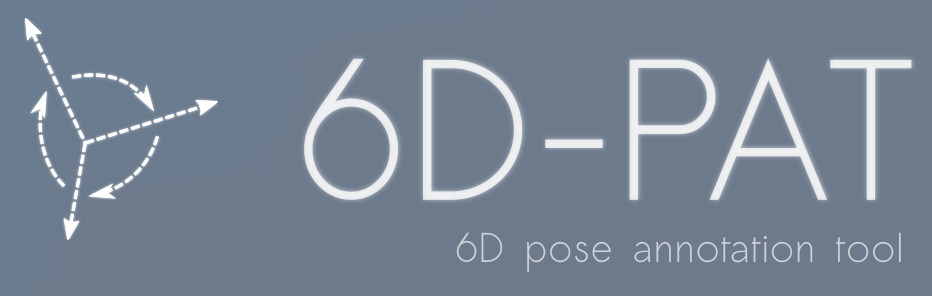
\includegraphics[width=0.8\linewidth]{6dpat}
    \caption{The logo of the pose annotation tool 6D-PAT.}
    	\label{fig:6dpat_logo}
\end{figure} 

The following chapter analyzes the manual 6D pose annotation process and its prerequisites. To this end, we define the necessary terminology and explain the workflow of recovering poses from images using the tool we developed. 

\section{Terminology} \label{section:terminology}

\textbf{Image.} An image $I$ is a 2D matrix of pixels. The pixel $u$ at position $(i, j)$ is referenced by the tuple $(x, y)$, where $x = j$ and $y = i$. The author of this work chose this notation over the row-major matrix indexing because images are often column-major indexed. \\

\noindent\textbf{Object Model.} An \textit{object model} (or \textit{3D model}) $O$ is composed of a set of points $M \subseteq \mathbb{R}^3$ and a set of triangles $T \subseteq M^3$, also called a mesh. The type of object is not restricted. In the T-Less dataset \cite{tless}, the objects are mostly screws and other hardware. \\

\noindent\textbf{6D Pose.} A \textit{6D pose} $P$ is the tuple $(R, t)$. $R$ is the $3\times 3$ rotation matrix and $t \in \mathbb{R}^3$ the translation vector used to transform an object model into camera coordinates (see Section \ref{objectcoordinates}). \\

\noindent\textbf{Correspondence.} A \textit{correspondence} $C$ is the tuple $(u, p)$, which captures the relation between a pixel $u$ of an image $I$ and a 3D point $p$ on the surface of an object model $O$. The pixel $u$ is the projection of $p$ onto the image plane using the camera matrix $K$ and a pose $P$. A pose can be recovered computationally if at least three correspondences are known (see Section \ref{objectcoordinates}). \\

\noindent\textbf{Segmentation Mask.} A \textit{segmentation mask} (or \textit{segmentation image}) $S$ for an image $I$ is a second image of the same size. Each position $(x, y)$ of the mask encodes the class of the pixel at $(x, y)$ in $I$. The set of classes can be defined arbitrarily. In the context of this work, each class represents a type of object model. The segmentation mask can be seen as the mapping $s(x, y) = q_i$ for a class set $Q = \{q_0, \cdots, q_n\}$. \\

\noindent\textbf{Ground-Truth.} A \textit{ground-truth pose} $\bar{P}$ is a 6D pose, which is always recovered by a human instead of a machine. The ground-truth pose is the best approximation of the rotation and translation of an object model $O$ visible in an image $I$. It is an approximation because there can be a discrepancy between the real world object and its digital 3D representation. Image conditions like lightning, motion blur, etc. might make it unfeasible to recover the perfect pose. Camera distortions and other influences in the photographs of the objects might also not be modeled correctly or not accounted for at all. But it must apply that the translation and rotation error of a ground-truth pose $\bar{P}$ are within a certain threshold. \\

\noindent\textbf{Depth Image.} A \textit{depth image} is an image $D$ belonging to an image $I$ of the same size that contains the distance $d$ between the camera and the surface for each pixel $u$ in $I$. Depth images can be obtained from stereo images or using special cameras and are often used in pose estimation and other computer vision tasks. A depth image can also be denoted by \textit{RGB-D}.

\begin{figure}[!tbp]
	\centering
	\begin{subfigure}[t]{0.47\textwidth}
	\centering
    	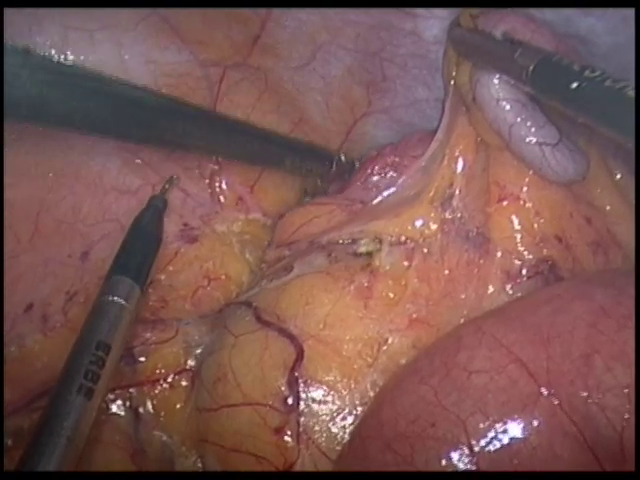
\includegraphics[width=0.8\linewidth]{sfb_original}
    	\caption{An example image from the Endoscopic Vision Challenge dataset. Image from \cite{endovis}.}
    	\label{fig:sfb_original}
	\end{subfigure}
	\hfill
	\begin{subfigure}[t]{0.47\textwidth}
	\centering
    	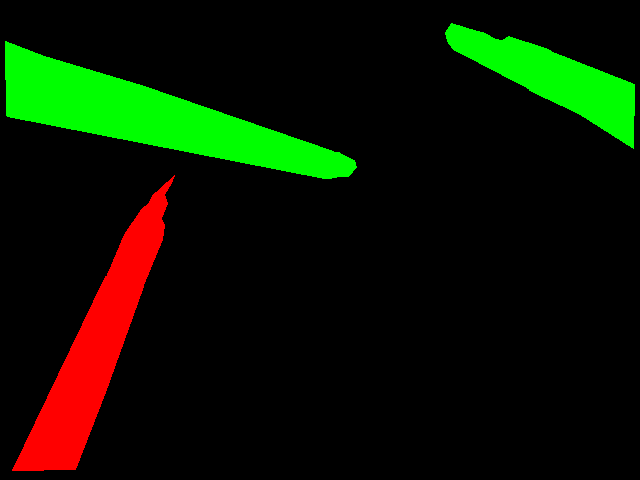
\includegraphics[width=0.8\linewidth]{sfb_segmentation}
    	\caption{The segmentation mask belonging to the image in fig \ref{fig:sfb_original}. The colors encode the tools' classes. Image from \cite{endovis}.}
    	\label{fig:sfb_segmentation}
	\end{subfigure}
	\caption{An example image and its corresponding segmentation mask from the Endoscopic Vision Challenge dataset.}
	\label{fig:sfb}
\end{figure} 

\section{Images of the Endoscopic Vision Challenge}

The goal of this work is to provide a system to successfully and efficiently annotate the images of the \textit{Endoscopic Vision Challenge} \cite{endovis}. The dataset includes segmentation masks but neither object models nor pose annotations or depth images. An example image together with the corresponding segmentation mask are given in \fig \ref{fig:sfb}. Occlusion and artifacts like motion blur can occur in the images. The issues with this dataset and the obstacles preventing its complete annotation are discussed Section \ref{section:6dpat_difficulties}. 

\section{6D Pose Annotation Tool (6D-PAT)}

The creation of sufficient training data for neural networks can be a time-consuming and tedious process. Using non-specialized tools designed for other purposes, like 3D modeling or CAD programs, require the person creating the annotations to get accustomed to complex user interfaces (\gls{ui}s). The goal of the annotation tool is to provide a system that allows easy and efficient annotation of images - images of the Endoscopic Vision Challenge in particular. The ground-truth poses recovered using the program can then be used to train a neural network. The program is written mainly in the language C++ and named \textit{6D - Pose Annotation Tool (\gls{6dpat})}. Its logo can be seen in \fig \ref{fig:6dpat_logo}. We developed the program on the \textit{Linux}-based operating system \textit{Ubuntu} but it is compatible to other operating systems, as well.

\subsection{Requirements}

%TODO re-read

Fulfilling the goal of providing a tool for annotating large datasets implies some requirements. Datasets can consist of thousands of images and many object models. To guarantee a fluid workflow, we need to provide the user with a browsable overview over the dataset. This prevents a disruptive annotation process, as the user doesn't need to open the next image or a different object model individually after recovering a pose. The program has to offer the possibility to select and view images and object models, respectively. The most essential part of such an annotation tool is the incorporation of functionality to recover poses and to edit misaligned poses. Different manual pose recovery mechanisms are possible. Due to the limited time frame of this work, we implemented only one method, which we expected to be the most efficient one.

\subsection{Frameworks \& Third-Party Libraries}

All necessary dependencies of the tool are listed below. The user needs to compile or install the dependencies before using the annotation tool. But since all frameworks and libraries are platform-independent, the program can be compiled and run on different systems. \\

\noindent\textbf{Qt.} \textit{Qt} \cite{qt} is a powerful framework for C++ that offers a vast selection of user interface components but also general functionality that exceeds the capabilities of the standard C++ library. Qt was also chosen as the main framework because it ensures portability of C++ applications by encapsulating system calls of all kind. \\

\begin{figure}[!tbp]
	\centering
	\begin{subfigure}[t]{0.47\textwidth}
		\centering
    	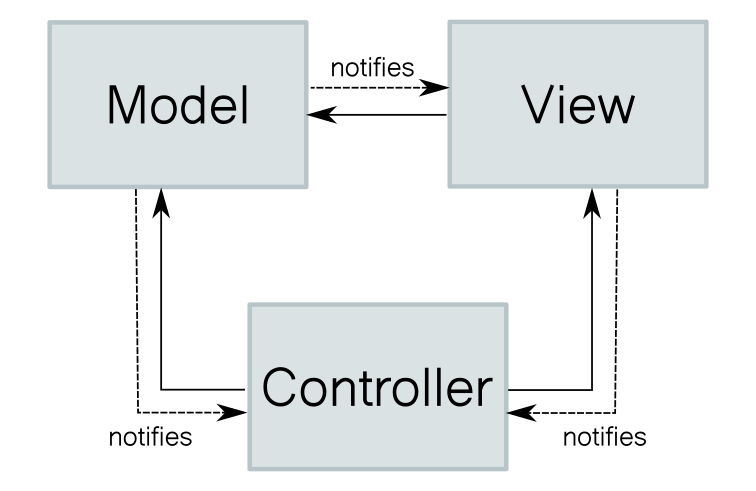
\includegraphics[width=0.8\linewidth]{mvc}
    	\caption{The Model-View-Controller architecture. The solid lines stand for a direct connection either because the target is owned or known by reference. The dashed line is an indirect connection realized using the observer pattern or the Qt Signals and Slots mechanism visible in \fig \ref{fig:qt_signals_slots}.}
    	\label{fig:mvc}
	\end{subfigure}
	\hfill
	\begin{subfigure}[t]{0.47\textwidth}
	\centering
    	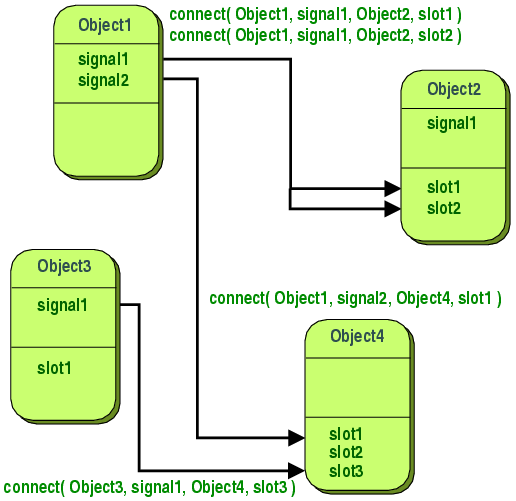
\includegraphics[width=0.8\linewidth]{qt_signals_slots}
    	\caption{The Signals and Slots mechanism of Qt. A class can define signals which can be emitted. Slots are functions that can be connected to signals. When a signal is emitted, all connected slots will be called. Image from \cite{qt_signals_and_slots}.}
    	\label{fig:qt_signals_slots}
	\end{subfigure}
	\caption{Two basic architectural concepts used in \gls{6dpat}: the model view controller pattern and the signal and slots pattern.}
\end{figure} 

\noindent\textbf{OpenGL.} \textit{OpenGL} \cite{opengl} is a widespread open-source 3D graphics library specification. Implementations of the specification exist for many different operating systems, which makes applications using OpenGL portable. \\

\noindent\textbf{OpenCV.} \textit{OpenCV} \cite{opencv} is a C++ library created for various computer vision tasks. OpenCV provides functions for object tracking, object detection, image segmentation and many more. We use its \textit{solvePnPRansac} method in this work. \\ 

\noindent\textbf{Assimp.} \textit{Assimp} \cite{assimp} is a C++ library designed to import 3D models. The library was incorporated into the tool to ensure a broad support of 3D model formats.

\subsection{Architecture \& Code Design}

\gls{6dpat} is primarily a UI program, i.e. its purpose is to display a window and enable optical interaction for the user, like clicking. Thus, we chose the \textit{Model-View-Controller (\gls{mvc})} pattern as the underlying architecture. \gls{mvc} separates the concerns of data management (Model), displaying data (View) and high level logic (Controller). The schematic of the \gls{mvc} architecture is shown in \fig \ref{fig:mvc}. The indirect connections are realized via Qt's signals and slots mechanism, which is visualized in \fig \ref{fig:qt_signals_slots}. To speed up interface creation, we used \textit{Qt Designer} to layout the views. Qt Designer is a graphical tool that allows placement of UI components and linking of signals and slots without directly writing code and is part of the standard Qt framework.

\begin{figure}[!tbp]
       \centering
   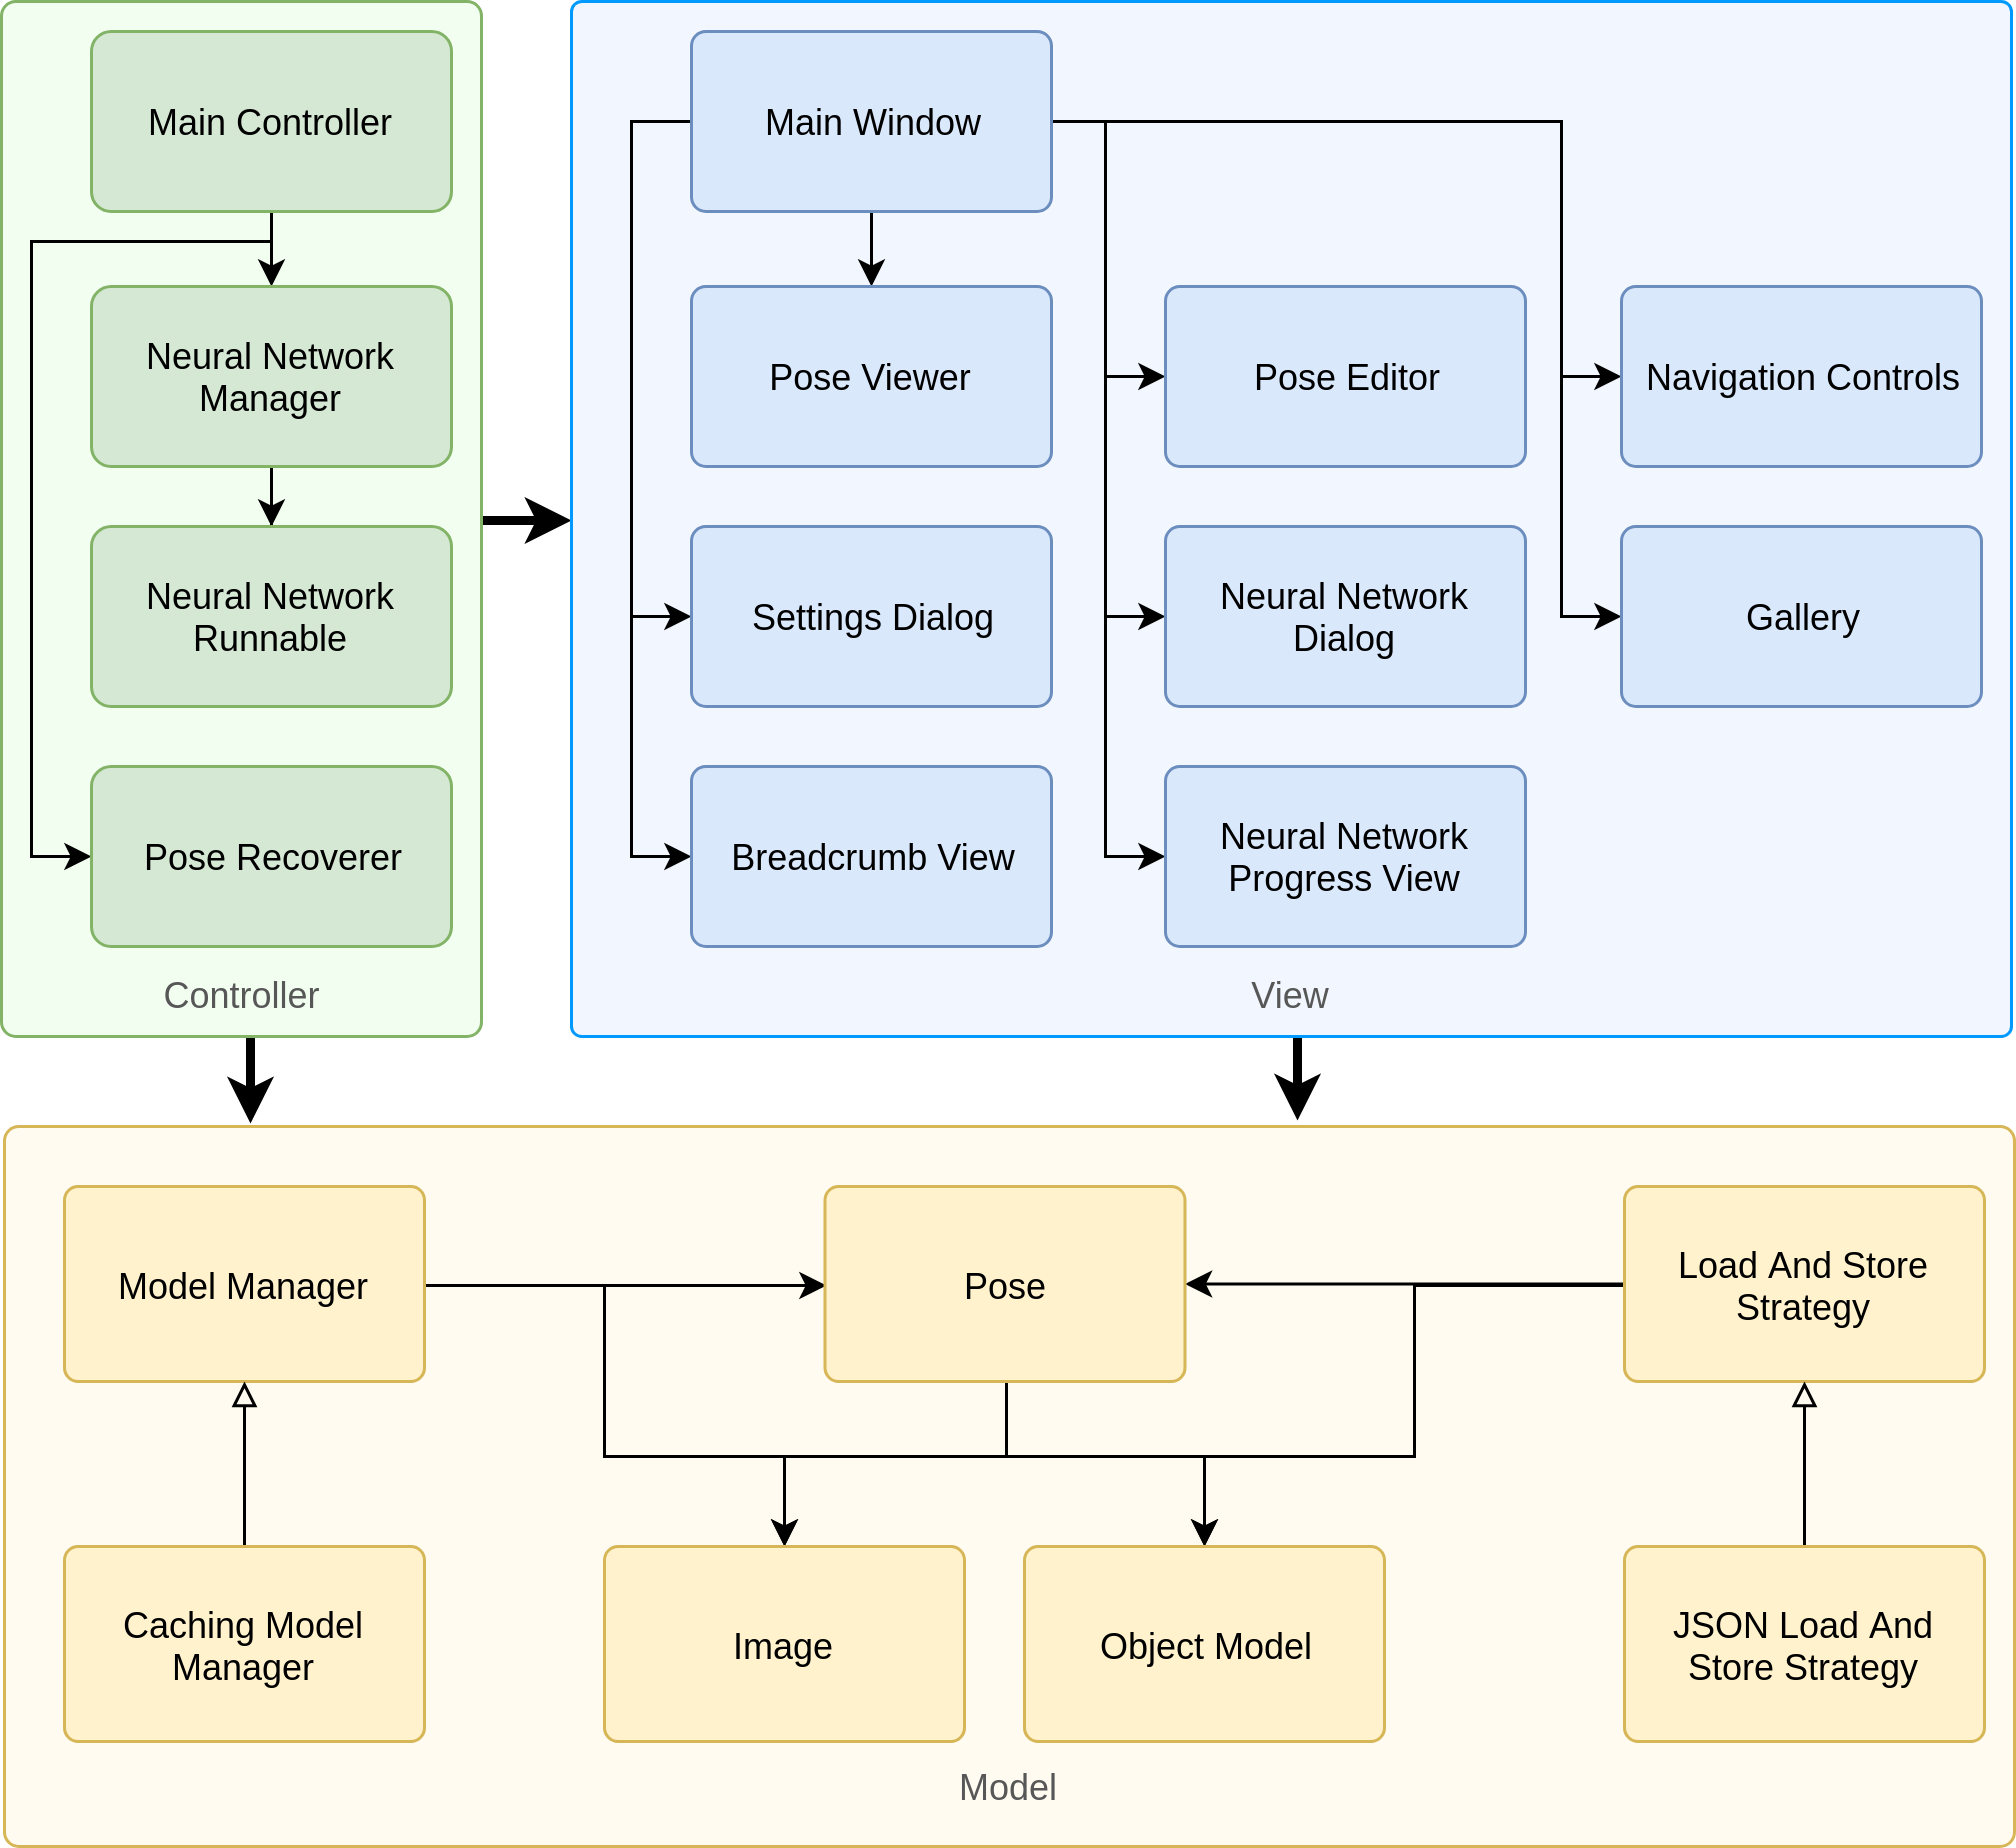
\includegraphics[width=\linewidth]{6dpat_class_diagram}
    \caption{An abstract high-level class diagram of a subset of the classes of \gls{6dpat}. The large rectangles show the affiliation of a contained class in the MVC pattern. Arrows between those rectangles imply which class can use which target class, although not all classes of the source rectangle necessarily use all classes of the target rectangle. Small filled-out arrows imply a use relationship, while the not filled-out arrow heads indicate inheritance.}
   \label{fig:6dpat_class_diagram}
\end{figure}

The most important classes of the program are displayed in \fig \ref{fig:6dpat_class_diagram}. The diagram is simplified for easier understanding. The large rectangles group the classes by their affiliation in the MVC pattern. The bold arrows between the groups denote which classes can use or know which other classes. This does not necessarily mean, that all classes of the source rectangle use all classes of the target rectangle. 

\subsubsection{Controller Classes}

The controller classes consist mostly of the \textit{Main Controller}, which owns the \textit{Pose Recoverer} and the \textit{Neural Network Manager}. The code of these classes has not been incorporated into the main controller to further separate the classes by concern and facilitate future modifications. The pose recoverer handles the clicked 2D-3D correspondences and offers functionality to compute the pose. The neural network manager handles all tasks of the network. To keep the UI responsive during time-consuming network operations, the network manager uses the \textit{Neural Network Runnable} to run tasks in a separate thread. This design allows easy substitution of how to the network is currently run, if necessary. The main controller also creates the \textit{Model Manager} and the \textit{Load And Store Strategy}. To use different implementations of either class, the controller has to be adjusted create those instead. The \textit{Main Window} receives the created model manager from the main controller

\subsubsection{View Classes}

The main controller creates the main window, which holds all views of the UI. It is the central view counterpart for the main controller and delegates all alterations requested by the controller to the other views. All signal and slots that are necessary between view classes get connected by the main window. Most of the signals and slots communication takes place between the \textit{Pose Viewer}, the \textit{Pose Editor} and the galleries. Whenever the user clicks an image or an object model in the gallery, the gallery notifies the viewer and editor to display the respective entity. The view classes know the model classes, especially the \textit{Model Manager}, by reference. For this end, the main window passes the model manager reference it received from the main controller to the other view classes.

\subsubsection{Model Classes}

The classes that contain the the paths to the data are the \textit{Image} class and the \textit{Object Model} class. The image also contains the camera matrix $K$. The \textit{Pose} class references an image and an object model and the respective rotation matrix $R$, as well as the translation vector $t$. The model manager and the load and store strategy interfaces were abstracted from the implementations \textit{Caching Model Manager} and \textit{JSON Load And Store Strategy} with extensibility in mind. This way, the strategy can be adapted to use a database instead of a JSON file, for example.

\subsubsection{Miscellaneous Classes}

Some classes are not displayed in \fig \ref{fig:6dpat_class_diagram}. We created a dedicated class to store the current settings of the program. This ensures compatibility between classes whenever the number of parameters of the settings or their type changes.

\subsection{Manual Annotation} 

This section describes the user interface of \gls{6dpat} and the steps required to annotate images with 6D poses. 

\subsubsection{Preparation}

\begin{figure}[!tbp]
	\centering
	\begin{subfigure}[t]{\textwidth}
		\centering
    	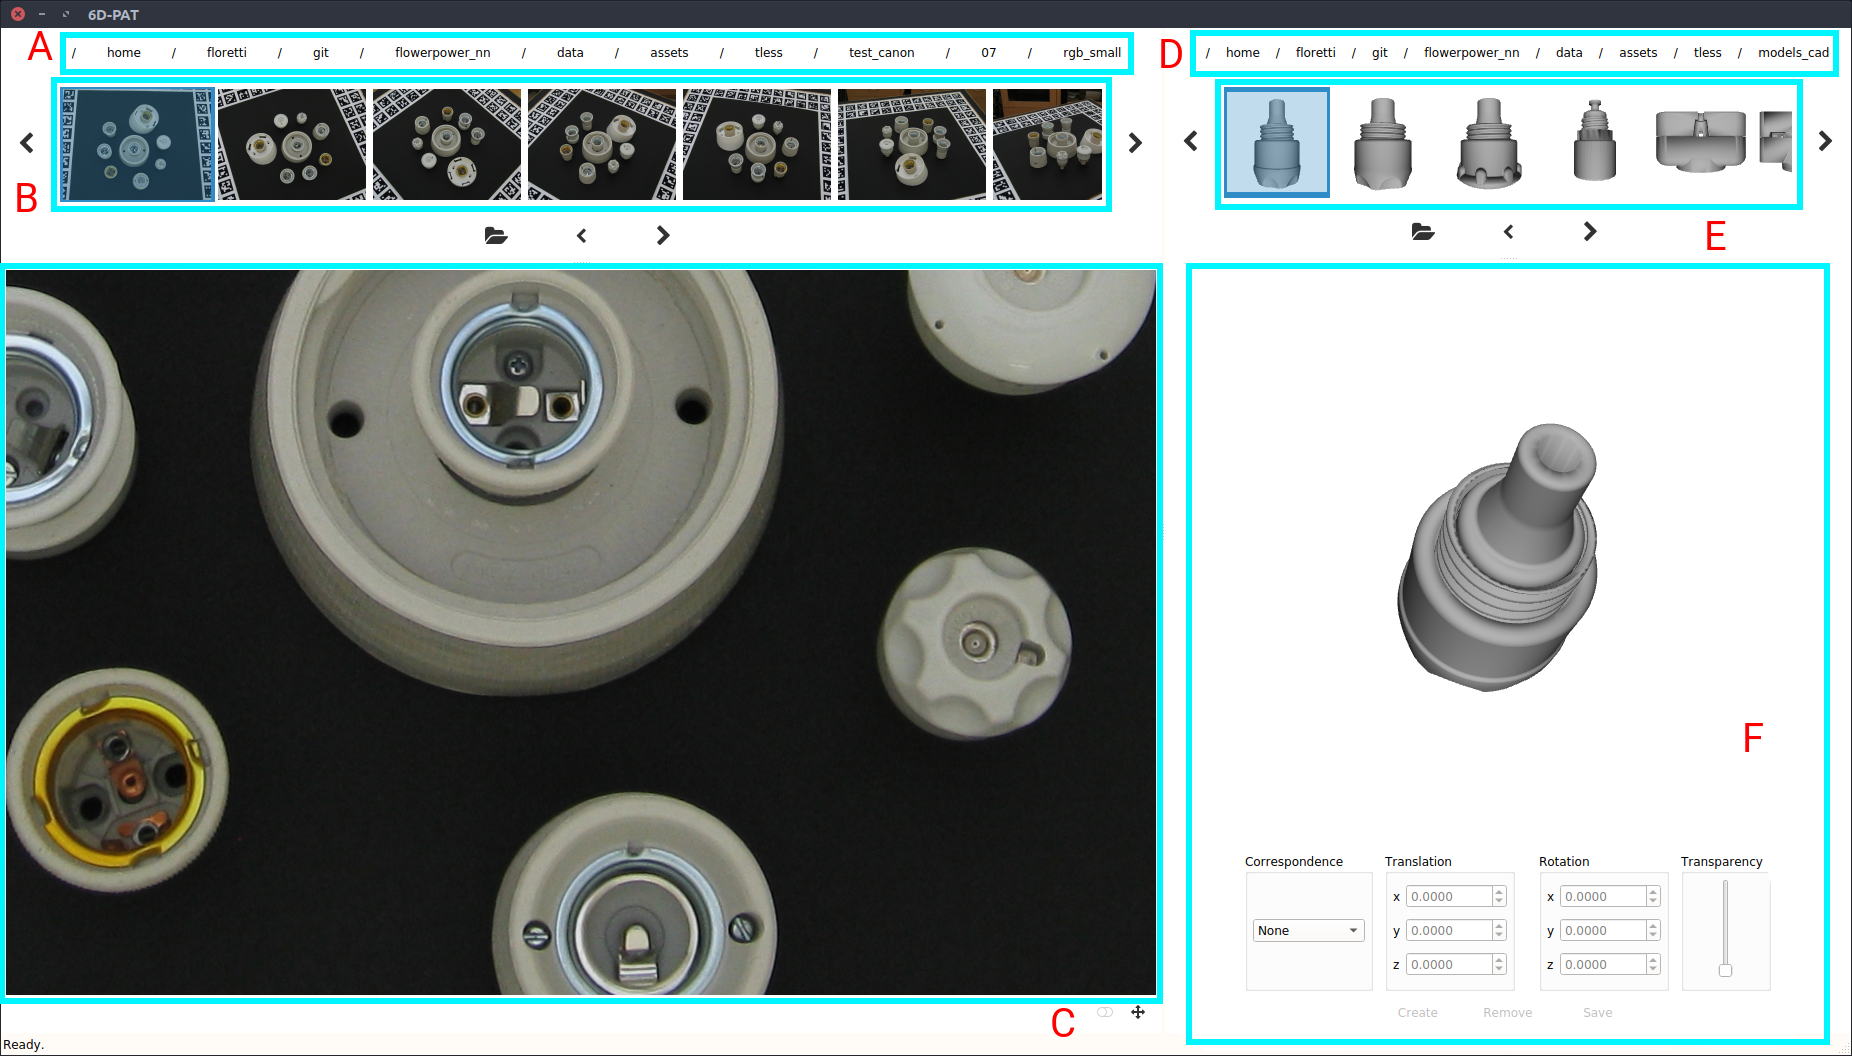
\includegraphics[width=\linewidth]{6dpat_components}
    	\caption{The user interface of the annotation tool \gls{6dpat}. The displayed images and object models are from the T-Less dataset. The following components are marked with a turquoise box: \textbf{A}: The full path of the currently selected folder to load images from. \textbf{B}: The \textit{Images Gallery} showing the images loaded from the selected path. \textbf{C}: The \textit{Pose Viewer} shows the image selected in gallery B. The user can click on the image to define the 2D starting point of a correspondence. \textbf{D}: The full path of the currently selected folder to load object models from. \textbf{E}: The \textit{Objects Gallery} of rendered 3D previews of the object models loaded from the selected path. \textbf{F}: The \textit{Pose Editor} shows the object model selected in gallery E. The user can click on the object model to complete the correspondence with the 3D point. The controls at the bottom can be used to edit existing poses.}
    	\label{fig:6dpat_components}
	\end{subfigure}
	\par\bigskip
	\begin{subfigure}[t]{0.47\textwidth}
		\centering
    	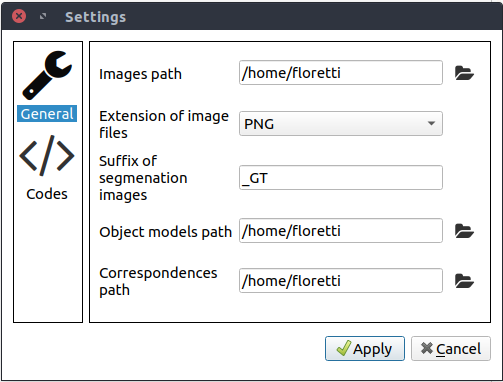
\includegraphics[width=\linewidth]{6dpat_settings}
    	\caption{The settings dialog of \gls{6dpat}. The dialog allows editing of the paths where the program loads images, object models and poses from.}
    	\label{fig:6dpat_settings}
	\end{subfigure}
	\hfill
	\begin{subfigure}[t]{0.47\textwidth}
	\centering
    	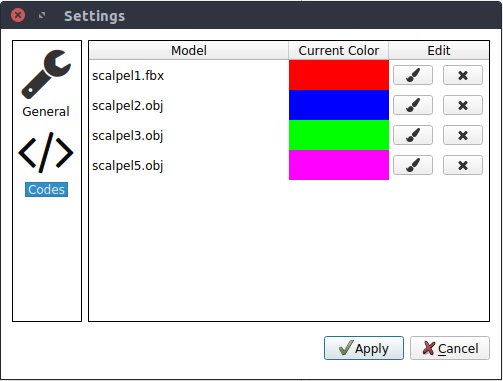
\includegraphics[width=\linewidth]{6dpat_settings_codes}
    	\caption{The tab of the settings dialog that can be used to assign colors to the object models.}
    	\label{fig:6dpat_settings_codes}
	\end{subfigure}
	\caption{The UI of \gls{6dpat}.}
	\label{fig:6dpat_ui_overview}
\end{figure}

The first step after starting the program is to open the settings (see \fig \ref{fig:6dpat_settings}) and to set the path to the images that are to be annotated, as well as the path to the folder that contains the object models that are visible in the images. 

The folder of the images has to contain a JSON file that holds the camera matrix $K$ for each individual image. If no camera info file exists, a Python script that is distributed with the neural network can be used to created approximate camera matrices. The path to the segmentation images, if any, has to be set as well. The program loads the images and the segmentation images and sorts them by the numbers in their filenames and matches image $I$ at index $j$ with the segmentation image $S$ at index $j$. 

Lastly, the user needs to specify the location of the JSON file where the program is supposed to load existing ground-truth poses from and write new ones to. If no such file exists, an empty one can be created and selected. If segmentation images are present, they are linked to the respective image and can be viewed by activating the toggle at the bottom right corner of the pose viewer. The program displaying a segmentation image can be seen in \fig \ref{fig:sfb_segmentation}. 

If required, the user can assign colors to the object models using the settings dialog depicted in \fig \ref{fig:6dpat_settings_codes}. The colors should correspond to the color used in the segmentation mask. The object models gallery will automatically display only the object models whose color is present in the segmentation image of the currently viewed image. If no segmentation images exist, the gallery shows all object models.

\subsubsection{Creation of Correspondences and Pose Recovery} \label{subsection:correspondence_and_pose_creation}

\begin{table}
\centering
    \begin{tabular}{|c||ccccc|} \hline
\diagbox{\# Object}{Image} & 0000.jpg & 0150.jpg & 0250.jpg & 0350.jpg & 0500.jpg \\ \hline\hline
01           &  2:30 min & 1:23 min & 2:05 min & 3:06 min & 0:50 min \\ 
        15 & 2:16 min & 1:51 min & 1:35 min & 2:20 min & 3:07 min \\ \hline
\end{tabular}
	\caption{The table shows the time the author needed to recover a single pose in an image using 6D-PAT. Images were taken from test scene 7 of the T-Less dataset. The measurements shall give an impression of the tool's efficiency, without making the claim to resemble an empirical study.} 
	\label{tabel:6dpat_example_times}
\end{table}

The component corresponding to the letters that we use in the following paragraph can be taken from \fig \ref{fig:6dpat_components}. To annotate a new pose, the user has to select an image $I$ from the images gallery (see \textit{B} in \fig \ref{fig:6dpat_components}) first. The pose viewer (see \textit{C} in \fig \ref{fig:6dpat_components}) then displays the image. Gallery \textit{E} is used to select the object model $O$ that the image is to be annoated with. The pose editor (see \textit{F} in \fig \ref{fig:6dpat_components}) shows the selected object model. The user can rotate the object to view otherwise hidden areas. Using the arrow keys, the user can move the object along the $x$ and $y$ axis and also, if the shift key is pressed, along the $z$ axis. 

When the object is in an appropriate position, the user can begin to create a correspondence $C$ by clicking on $I$. This defines the 2D location $u$ of the correspondence. To complete the correspondence, the object model $O$ has to be clicked at the respective position $p$. This procedure has to be repeated until enough correspondences $C_1, \cdots, C_n$ have been defined to recover the new pose $P$. The minimum number of correspondences is $4$. 

The creation process is shown in \fig \ref{fig:6dpat_correspondence_creation}. More correspondences can make the initial pose more accurate. Clicking the \textit{Create} button at the bottom of the pose viewer creates the pose $P$ using the correspondences $C_i$ and OpenCV's \textit{solvePnPRansac} method. The newly created pose can be refined using the controls of the pose viewer. After pose refinement, it is necessary to click the \textit{Save} button. 

The slider labeled \textit{Transparency} can be used to reduce the object's opacity on the image. After all poses have been annotated successfully, the next image can be selected from the image gallery. This operation has to be repeated until the dataset is fully annotated, although intermediate states can already be used to train the network (see Chapter \ref{chapter:semi_automatic}).

It is possible to use the neural network to predict poses. This requires proper setup and training of the network beforehand. The user can then start the prediction process by clicking the \textit{Predict} button in the lower right corner of the pose editor.

%TODO rewrite and provide example images
Example times of the manual annotation process (without aid of the network) are given in Table \ref{tabel:6dpat_example_times}. The measured times were achieved by the author of this work trying to recover a single pose of the specified object model. The discrepancy between the measurements depends on the computed initial pose. A view that shows the object along multiples axes works best because defining correspondences along those axes fixes the rotation.

We gave this way of recovering poses preference over other possible techniques for multiple reasons. Another intuitive way of recovering poses is dragging the object model from the pose editor onto the pose viewer at the approximately correct position. We assumed that the chosen procedure is faster, because when enough precise corerspondences are clicked, rotation and position are accurate immediately.

\begin{figure}[!tbp]
	\centering
    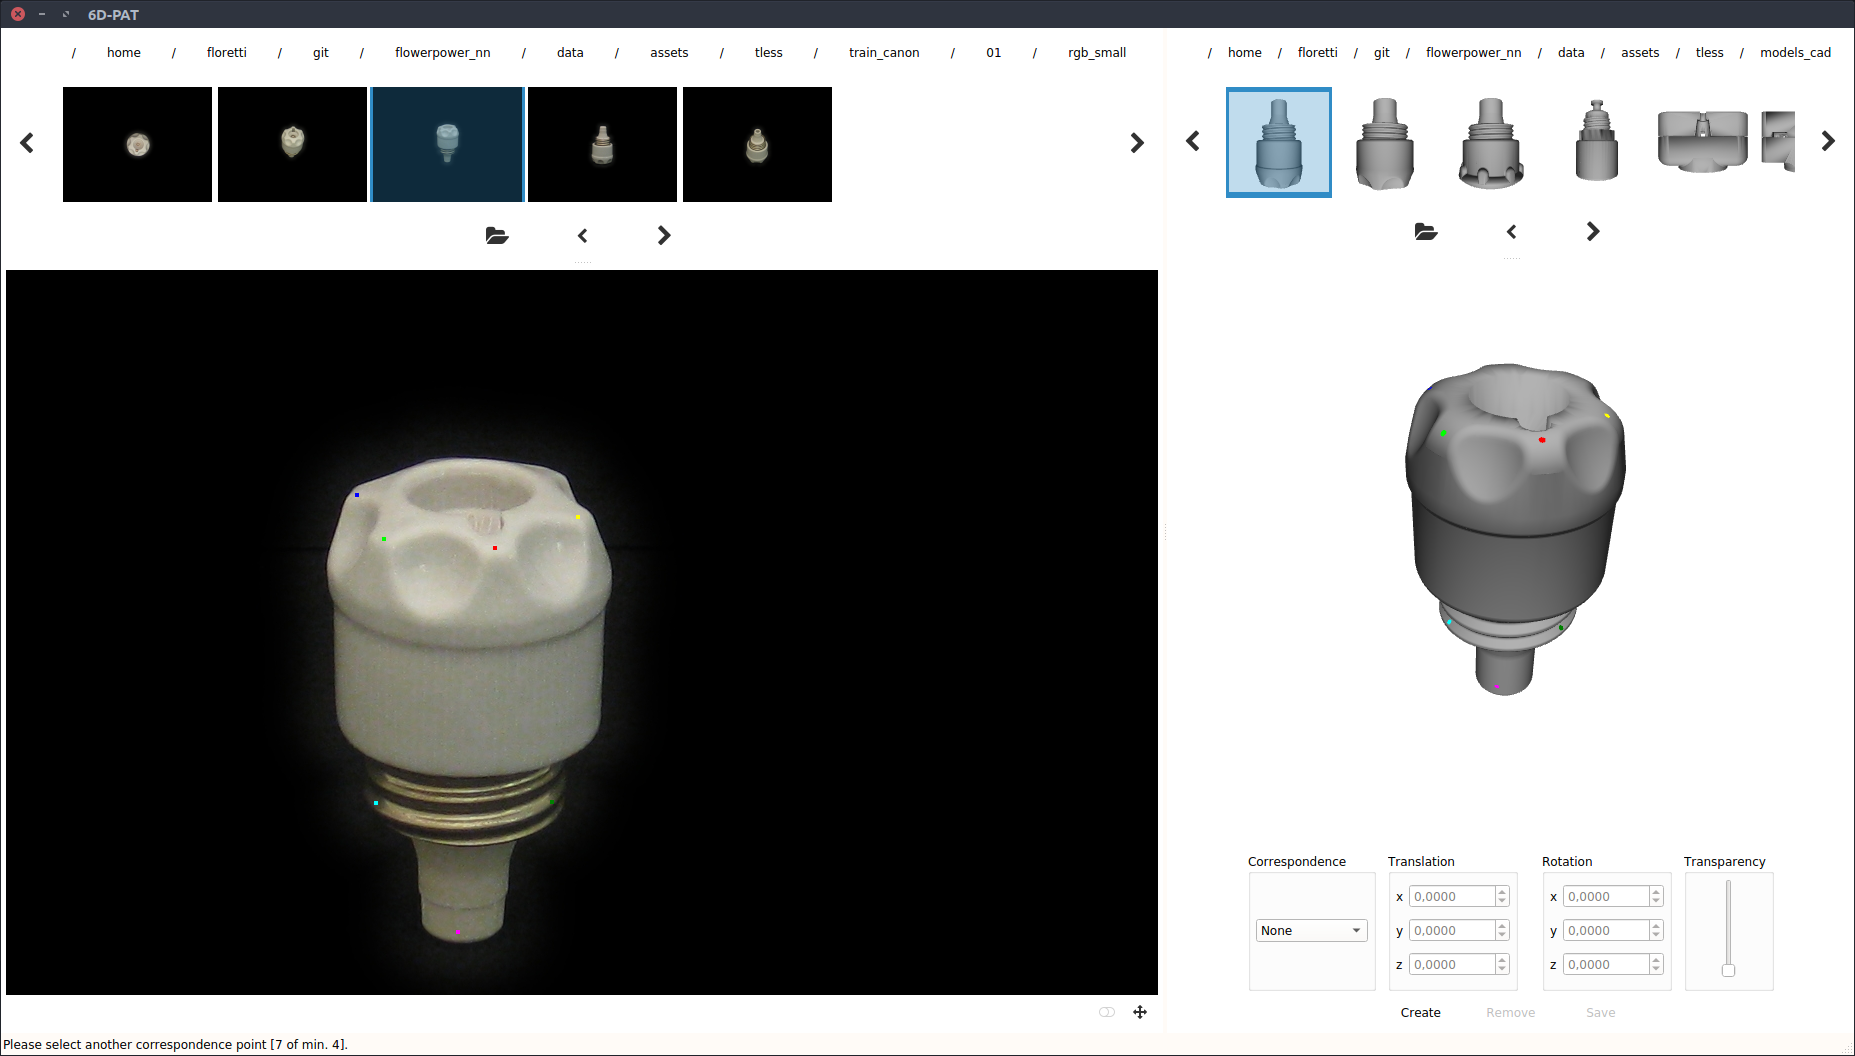
\includegraphics[width=\linewidth]{6dpat_correspondence_creation}
    \caption{The pose creation process. The user has to click the image first and then the corresponding 3D location on the object model. The red circles and red lines were added afterwards to emphasize the colored dots drawn by the program.}
    \label{fig:6dpat_correspondence_creation}
\end{figure} 

\subsection{Problems \& Difficulties} \label{section:6dpat_difficulties}

%TODO re-read

During the implementation of the program, multiple problems arose and complicated the development process. We summarize the most important ones and explain issues which impacted the final design.

One of the major factors that prolonged the implementation process was utilizing the \textit{Qt3D} framework, which is part of the main Qt framework, to realize all graphical processing. Qt3D's purpose is to encapsulate graphics programming to increase portability of applications including 3D graphics. The incomplete documentation and unintuitive concepts make it difficult to use without consultation. After complications still emerged in the almost completed annotation tool, the Qt3D framework was deemed unusable and omitted in favor of a native OpenGL implementation.

Initially, a desired feature was to present another unannotated image after the user finished annotating all poses in the current image. This is not feasible for multiple reasons. First of all, a user might still not be content with the poses. Selecting the next image programmatically could happen too early and thereby disrupt the annotation process of the user.

The datasets can also have very distinct characteristics, which require the user to choose the next image manually. For a dataset like T-Less, many images have to be skipped due to their similarity. A network trained on one view on an object only, will likely predict inaccurate poses for a different view showing other characteristics of that object. The support of an accurate network in the annotation process can be used as a motivation for the user.

The diversity of available datasets (see Chapter \ref{chapter:experiments} for a selection of datasets) is also the reason why the program does not provide functionality to initialize the next poses based on the ones in the last image. This feature would imply too many assumptions on the dataset and, in the worst case, cause more work for the user. 

While trying to annotate the images of the Endoscopic Vision Challenge dataset, it became clear that proper 3D models are crucial for successful annotation. To temporarily annotate the medical images, 3D surgical tools were downloaded from the internet as a replacement for the missing object models. But having a different shape and also missing the distinctive features of the real objects makes it very difficult to estimate the ground-truth pose. The influence of contradicting annotated poses during training of a network is not clear. The author of this work strongly recommends to obtain the correct 3D models before annotating the Endoscopic Vision Challenge images. The issue of the object models not fitting the segmentation mask can be seen in \fig \ref{fig:sfb_segmentation}. \fig \ref{fig:sfb_original} shows the actual image and the discrepancy between the object models and image pixels.

\begin{figure}
	\begin{subfigure}[t]{0.47\textwidth}
		\centering
    	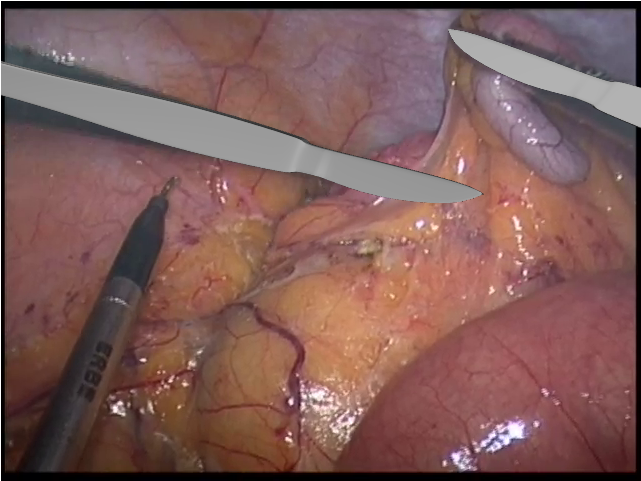
\includegraphics[width=\linewidth]{6dpat_sfb_image}
    	\caption{An image from the medical images dataset annotated using 6D-PAT. The correct rotation and translation are difficult to estimate without the correct 3D models.}
    	\label{fig:6dpat_sfb_image}
	\end{subfigure} 
	\hfill
	\begin{subfigure}[t]{0.47\textwidth}
		\centering
    	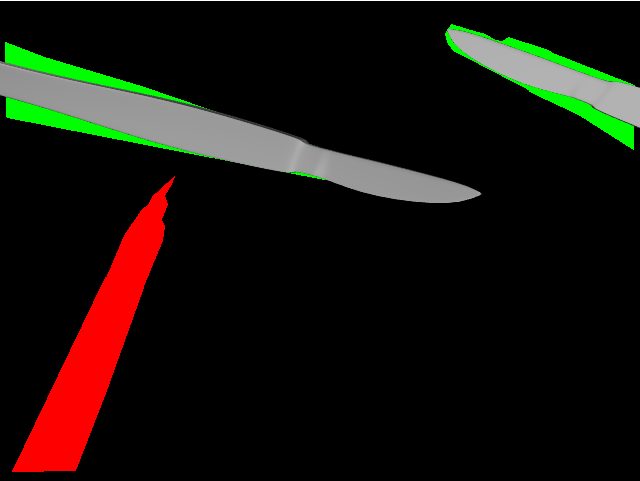
\includegraphics[width=\linewidth]{6dpat_sfb_segmentation}
    	\caption{The corresponding segmentation image to image \ref{fig:6dpat_sfb_image}. The discrepancy between the segmentation masks and the object model is the clearly visible green area.}
    	\label{fig:6dpat_sfb_segmentation}
	\end{subfigure} 
	\caption{Example annotations of images of the Endoscopic Vision Challenge dataset (originals depicted in \fig \ref{fig:sfb}). The object model is taken from \cite{3d_scalpel_online}.}
	\label{fig:6dpat_sfb}
\end{figure} 

A first try to use the official Python bindings did not work to our complete satisfaction. Including the bindings in the program required complex alterations to the program. Running Python scripts is also possible by starting a new process. Qt natively offers this functionality.

The Python binding is not complete, yet. Training is not possible and a deep learning expert has to setup the network and its parameters to enable its usage in the program. The current state of the incorporation of the network is to be seen as a proof of concept that requires further development.

Because the neural network is trained for one object only, the time-intensive step (proportional to the overall time needed for inference on one image) of loading the trained weights has to be performed before predicting poses for different objects. The frame of this work was to explore neural networks trained for one object only, it is therefore not known whether this overhead of loading the weights can be reduced.

\subsection{Future Improvements of 6D-PAT}

%TODO re-read

To provide an outlook how the program can be improved in the future, we mention solutions to some of the problems of Section \ref{section:6dpat_difficulties}. An important feature that should be implemented is allowing to move the object models around on the displayed image by dragging and rotating them using the mouse. The initial poses using the clicking procedure are already sufficiently accurate in many cases. But when the camera is looking along an axis of the object, the rotation can be far off. The user can correct these poses with the provided controls. The described editing process could profit from this functionality in terms of time needed per annotation. To provide the user with a better overview of the image and its annotated poses, a zoom option should be implemented, as well.

The binding of the neural network to the program does not allow to load the weights of the net and persist this state in the memory of the computer. In case that the user wants to annotate a large dataset of just one object, they could profit from a feature allowing to keep the weights in memory instead of loading them each time the inference process is started. This way, predicting the pose for only one image could be achieved in significantly less time.

Another suggested step is to fully incorporate the network in the annotation tool. This way, inexperienced users can profit from the network without the need for an expert to run the network inference. There is probably no way to automatize setting up the network, as this requires knowledge of neural networks. In an ideal setting, this interference can be reduced to a minimum and users are introduced to the most relevant parameters only, which they can set from within the program.